% Created 2022-03-16 Wed 12:55
% Intended LaTeX compiler: pdflatex
\documentclass[presentation]{beamer}
\usepackage{listings}
\usepackage[utf8]{inputenc}
\usepackage[T1]{fontenc}
\usepackage{graphicx}
\usepackage{longtable}
\usepackage{wrapfig}
\usepackage{rotating}
\usepackage[normalem]{ulem}
\usepackage{amsmath}
\usepackage{amssymb}
\usepackage{capt-of}
\usepackage{hyperref}
\usetheme{Warsaw}
\hypersetup{
colorlinks=true,%
urlcolor=blue,%
linkcolor=blue%
}
\usepackage[gen]{eurosym}    % For € symbol
\usepackage{wasysym}         % For smileys
\usepackage{bclogo}          % For bcattention & bccrayon signs
\usepackage{fontawesome}     % For pretty UTF-8 emojis \faWarning \faExclamationTriangle
\usepackage{tikz}            % For drawings
\usetikzlibrary{arrows.meta} % For arrow heads
\usetikzlibrary{shadows}
\usepackage{tikzsymbols}     % For Sticky man
\usepackage{listings}        % To insert Java code listing
\definecolor{dkgreen}{rgb}{0,0.6,0}  %% Colors for the Java listings
\definecolor{gray}{rgb}{0.5,0.5,0.5}
\definecolor{mauve}{rgb}{0.58,0,0.82}
\lstset{frame=none,          % For Java listings
language=java,
aboveskip=1mm,
belowskip=1mm,
showstringspaces=false,
columns=flexible,
basicstyle={\scriptsize \ttfamily},
numbers=left,
numberstyle=\scriptsize\color{gray},
keywordstyle=\color{blue},
commentstyle=\color{dkgreen},
stringstyle=\color{mauve},
breaklines=true,
breakatwhitespace=true,
tabsize=2
}
\setbeamercolor{normal text}{fg=white,bg=black!90}
\setbeamercolor{structure}{fg=white} %% TODO Problem with "description" env!
\setbeamercolor{alerted text}{fg=red!85!black}
\setbeamercolor{item projected}{use=item,fg=black,bg=item.fg!35}
\setbeamercolor*{palette primary}{use=structure,fg=structure.fg}
\setbeamercolor*{palette secondary}{use=structure,fg=structure.fg!95!black}
\setbeamercolor*{palette tertiary}{use=structure,fg=structure.fg!90!black}
\setbeamercolor*{palette quaternary}{use=structure,fg=structure.fg!95!black,bg=black!80}
\setbeamercolor*{framesubtitle}{fg=white}
\setbeamercolor*{block title}{parent=structure,bg=black!60}
\setbeamercolor*{block body}{fg=black,bg=black!10}
\setbeamercolor*{block title alerted}{parent=alerted text,bg=black!15}
\setbeamercolor*{block title example}{parent=example text,bg=black!15}
\setbeamertemplate{navigation symbols}{}
\setbeamertemplate{headline}{}
\addtobeamertemplate{navigation symbols}{}{%
\usebeamerfont{footline}%
\usebeamercolor[fg]{footline}%
\hspace{1em}%
\insertframenumber{}/\inserttotalframenumber{}
}
\AtBeginSection[]
{
\begin{frame}<beamer>
%\frametitle{Outline for section \thesection}
\tableofcontents[currentsection]
\end{frame}
}
\newcommand{\myarrow}[6]{ % size / src / linestyle / text / arrowhead / dest
\begin{tikzpicture}[baseline=-0.5ex]{
\node[inner sep=0](@1) at (0,0) {#2};
\node[inner sep=0](@2) at (#1,0) {#6};
\draw [#3,arrows={#5},shorten >= 2pt,shorten <= 2pt] (@1) -- (@2) node[pos=.5,above,inner sep=1pt] { #4 };}
\end{tikzpicture}\xspace
}
\def\up#1{$^\text{#1}$}
\newcommand{\FrFlag}{\includegraphics[height=1.5em]{../images/UML/Lecture1/flag_france.png}}
\newcommand{\LOTRing}{\includegraphics[height=1.5em]{../images/UML/Lecture1/LOTR_1Ring.png}}
\usetheme{default}
\author{Guillaume MULLER}
\date{\today}
\title{High Performance Programming -- SIMD -- Intro}
\title[HPP -- SIMD -- Intro]{High Performance Programming\\SIMD Intro -- MMX/SSE/AVX}
\subtitle{FISE2-INFO2}
\hypersetup{
 pdfauthor={Guillaume MULLER},
 pdftitle={High Performance Programming -- SIMD -- Intro},
 pdfkeywords={High-Performance Programming SIMD Introduction MMX SSE AVX},
 pdfsubject={High Performance Programming -- SIMD -- Intro},
 pdfcreator={Emacs 26.3 (Org mode 9.5.2)}, 
 pdflang={English}}
\begin{document}

\maketitle

\section*{}
\label{sec:org463391e}

\begin{frame}[label={sec:org2754b3a}]{Why having HPP lectures in FISE2? Why HPP?}
\pause
\begin{block}{Classical approach to HPP = distribute on cluster}
\begin{itemize}
\item What if the initial code is inefficient?
\item \(\Rightarrow\) Optimize locally / Think parallel
\end{itemize}
\pause
\end{block}
\begin{block}{Current machines already are massively parallel}
\begin{itemize}
\item Multi-Core, Multi-Thread\ldots{}
\end{itemize}
\pause
\end{block}
\begin{block}{A large part of optimizations can not be treated automatically}
\begin{itemize}
\item \(\Rightarrow\) impossible to rely on tools written by others
\item \(\Rightarrow\) as (future) engineers in CS: mandatory knowledge
\end{itemize}
\end{block}
\end{frame}

\begin{frame}[label={sec:org2c4cc7f}]{Why SIMD/MMX/SSE/AVX?}
\begin{block}{Task Parallelism}
\begin{itemize}
\item Execute coarse-grained pieces of code on \(\neq\) pieces of hardware
\item Multi-Cores, \alert{Multi-Threading}\ldots{}
\end{itemize}
\pause
\end{block}
\begin{block}{Instruction/Data Parallelism}
\begin{itemize}
\item Tiny pieces of code/data simultaneously on = hardware
\item \alert{SIMD}
\end{itemize}
\pause
\end{block}

\begin{block}{ ~~}
\medskip
\begin{itemize}
\item Write a code that is \alert{highly efficient}
\begin{itemize}
\item because \alert{highly adapted to hardware}
\item (thus less portable)
\end{itemize}
\end{itemize}
\medskip \pause
\begin{itemize}
\item \emph{Who has already used/programmed a processor \(\neq\) Intel?}
\end{itemize}
\bigskip
\end{block}
\end{frame}


\begin{frame}[label={sec:orga7b25b0}]{"Ça dépend" ("ça dépasse"?)}
\definecolor{myblue}{HTML}{9999FF}
\scalebox{.72}{
\begin{tikzpicture}[x=3cm,y=1.5cm]
   %\pgfpointxy{1}{1}
   % Styles
   \tikzset{rnode/.style={draw,rectangle,rounded corners=3pt,drop shadow,fill=myblue}}
   \tikzset{sarrow/.style={very thick,->,>=stealth'}}

   \node[rnode] (Designer)    at (2,0)  { \parbox{3.5cm}{ \center { \bf Designer } \\ Micro-Architecture } } ;

   \onslide<2-> { \node[rnode] (Past)        at (0,0)  { \parbox{3.5cm}{ \center { \bf \large Past }       \\ { \normalsize \begin{itemize} \item Needs \item Capacities \item Errors \end{itemize} } } } ; }
   \onslide<2-> { \node[rnode] (Future)      at (4,0)  { \parbox{3.5cm}{ \center { \bf \large Future }     \\ { \normalsize \begin{itemize} \item Dreams \item New needs \item New Capacities \end{itemize} } } } ; }
   \onslide<3-> { \node[rnode] (Users)       at (2,+2) { \parbox{3.5cm}{ \center { \bf \large Users }      \\ { \normalsize \begin{itemize} \item Developers \item Compilers \end{itemize} } } } ; }
   \onslide<3-> { \node[rnode] (Electronics) at (2,-2) { \parbox{3.5cm}{ \center { \bf \large Electronics} \\ { \normalsize \begin{itemize} \item Physical Limits \item Complexity \end{itemize} } } } ; }

   \onslide<2-> { \draw[sarrow] (Past)     -> (Designer) ; }
   \onslide<2-> { \draw[sarrow] (Designer) -> (Future) ; }
   \onslide<3-> { \draw[sarrow] (Users)    -> (Designer) ; }
   \onslide<3-> { \draw[sarrow] (Designer) -> (Electronics) ; }
\end{tikzpicture}
}

\begin{block}<4->{Typical answer in this course}
\center \large "\alert{ça dépend}"
\end{block}
\end{frame}

\begin{frame}[label={sec:orgf7e0255},fragile]{"Reminder"}
 \begin{center}
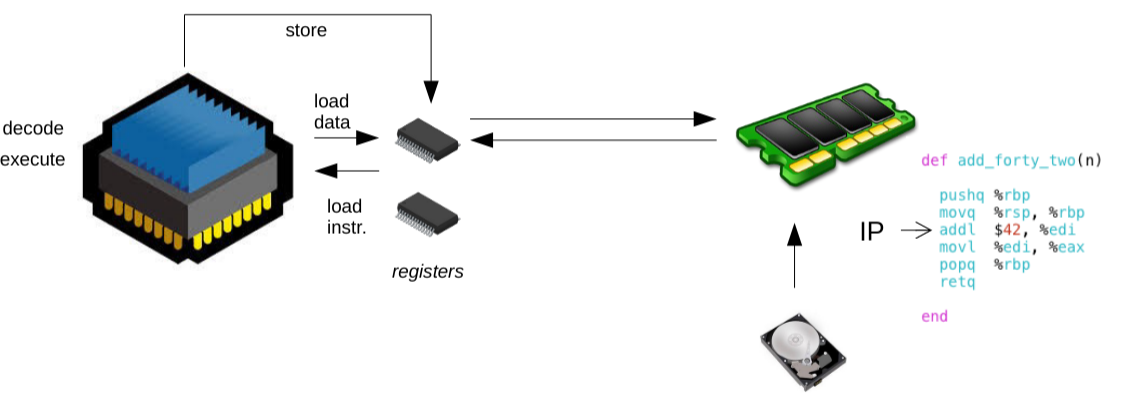
\includegraphics[width=.8\textwidth]{./images/cpu.png}
\end{center}
\pause
\begin{columns}
\begin{column}{.70\columnwidth}
\begin{block}{Instruction Types}
\begin{description}
\item[{\bf \black Flow}] \texttt{IP} / \texttt{JMP} \ldots{} \hfill
\item[{\bf \black Mem}] \texttt{LD} / \texttt{ST} \ldots{}  \hfill
\item[{\bf \black Calc}] \texttt{ADD} / \texttt{SUB} / \texttt{MULT} / \texttt{DIV} \ldots{} \hfill
\pause
\end{description}
\end{block}
\end{column}
\begin{column}{.29\columnwidth}
\begin{block}{Instruction Cycle}
\begin{itemize}
\item \small Fetch
\item \small Decode
\item \small Execute
\item \small Store
\item \small \ldots{}
\end{itemize}
\end{block}
\end{column}
\end{columns}
\end{frame}
\end{document}